\section{Git Static Object Model}

In this section we will show the specification in Alloy of the
git static object model. It will be mostly based on the textual
specification present in \cite{gitComm} and \cite{progit}.

\subsection{The objects}

All objects are identified by a sha defined by their contents. \par
"All the information needed to represent the history
of a project is stored in files referenced by a 
40-digit {\bf "object name"}..." (page 7) \par

However Alloy has a mechanism to uniquely identify atoms, so 
we can use it instead of the sha. \par

The objects are defined as in \cite{gitComm} (page 7) 
"...and there are four different types of objects: "blob",
"tree", "commit", and "tag". "

\begin{lstlisting}
abstract sig Object {
}
sig Blob extends Object{}
sig Tree extends Object {}
sig Commit extends Object{}
sig Tag extends Object{}
\end{lstlisting}

``A ''blob`` is used to store file data - it is generally a file'' 
\cite{gitComm} (page 8). We can abstract from it.

"A "tree" is basically like a directory - {\bf it references a bunch
of other trees and/or blobs}..." (page 8)

\begin{lstlisting}
sig Tree extends Object {
	contains : Name -> one (Tree+Blob)
}
\end{lstlisting}

Again from \cite{gitComm}. \par 
"As you can see,a commit is defined by :
... \par
parent(s) : {\bf The SHA1 name of some number of commits which
represent the immediately previous step(s) in the 
history of the project}. The example above has one parent;
merge commits may have more than one. A commit with no 
parents is called a "root" commit, and represents the 
initial revision of a project. {\bf Each project must have at
least one root. A project can also have multiple roots,
though that isn't common (or necessarily a good idea)}". (page 12)

\begin{lstlisting}

sig Commit extends Object{
  points : Tree,
  parent : set Commit
}

sig RootCommit extends Commit{}

\end{lstlisting}

\begin{lstlisting}
fact {
  no ^parent & iden
  no RootCommit.parent
  all c : Commit - RootCommit | some c.parent	
}

\end{lstlisting}

One of the advantages of git compared to others VCS is the operation
of creating a new branch. While in others VCS, a copy of the hole project is
done each time we create new branch, in git, only a new pointer is created.

"A branch in Git is {\bf simply a 
lightweight movable pointer to one of these commits}." \par \cite{progit} 
(pag 39)
``The special pointer called {\bf Header 
points to the branch we are working on}''. \cite{progit} (pag 40)

\begin{lstlisting}
sig Branch {
	mark : Commit,
	head : lone Branch
}{
	some Commit <=> one head
}
\end{lstlisting}


\subsection{Implicit specifications}

As the book \cite{gitComm} says, a "tree" acts
like a directory, so we know that it or its 
descendants cannot point to themselves.

Also, git only deals with files and their paths. Thus, git cannot have
folders without descendants.

\begin{lstlisting}
let r = {x :Tree, y : Tree+Blob | 
		some n : Name | x->n->y in contains} {
	no ^r & iden
	all t : Tree | some t.r
}
\end{lstlisting}

A tree needs to have at most one parent. Because it is part
of a file's path.
\begin{lstlisting}
all t:Tree | lone contains.t
\end{lstlisting} \par

Only with this specifications we can already see some interesting examples, 
like the next one.\par

\begin{figure}[h!]
	\caption{A simple commit}
  \centering
    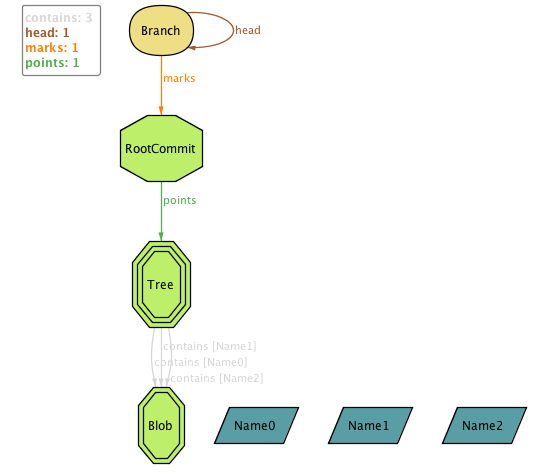
\includegraphics[scale=0.65]{images/image1.png}
\end{figure}

\pagebreak
\section{Index}

\subsection{The notion of path}

A path here is defined as part of a filesystem path. 
Each file on git has a blob and a path associated. 
The later and it's parents define a filesystem path.

\begin{lstlisting}
sig Path {
	pathparent : lone Path,
	name : Name,
	blob : lone Blob,
}
\end{lstlisting}

With this new information we introduce some new invariants.
We can't have cycles and two paths with the same
name, as in unix filesytem.
Only the leafs of a path can have a file (blob) associated.

\begin{lstlisting}
fact {
	 no ^pathparent & iden
	 all disj p,p' : Path | p.pathparent = p'.pathparent
	 implies p.name != p'.name
	 no Path.pathparent & blob.Blob
}
\end{lstlisting}

\subsection{The notion of Index}

The definition of Index:
"...staging area between your working directory and your
repository. You can use the index to {\bf build up a set of 
changes that you want to commit together}. When you create
a commit, {\bf what is committed is what is currently in the
index, not what is in your working directory.}"
\cite{gitComm} (page 17). \par

"The index is a binary file (generally kept in .git/index) 
{\bf containing a sorted list of path names}, each with permissions and the
SHA1 of a blob object" \cite{gitComm} (pag 120). \par 

\begin{lstlisting}
sig Path {
	...
	index: lone Path
}
fact{
	no Path.parent & index.Path
}
\end{lstlisting}

The index relation will define which files are in the index. And we know that only
files can be in the index. \par

Also : ``The index {\bf contains all the information necessary to generate a single
(uniquely determined) tree object}'' \cite{gitComm} (pag 121). \par
This description tells us that the index saves a snapshot of the system,
not the differences !

What is the practical difference between the Index and the Working
Directory? The Working Directory is just the root folder of a repository,
that we work on. When we want to save something in a commit, we have to explicitly 
tell git to add that to the Index. Once added, it
will be saved in the git database at the next commit. If we don't want to save
something in a commit, we simply don't add it to the Index.

Now we can see a more complete model of git.

\begin{figure}[h!]
	\caption{A simple commit and a file}
  \centering
    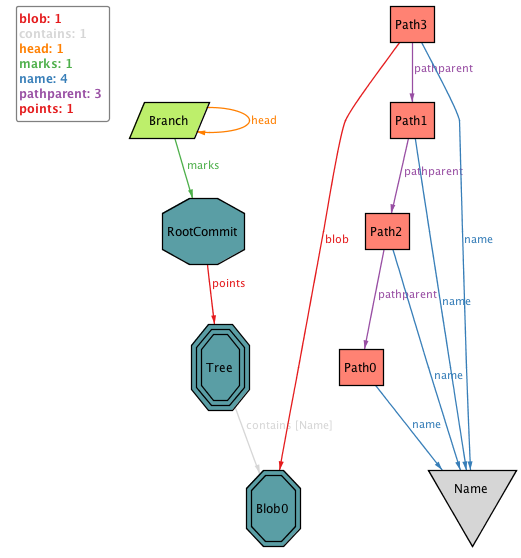
\includegraphics[scale=0.65]{images/image2.png}
\end{figure}

\pagebreak

